\section{Dataset Curation}

\begin{figure}[t]
    \centering
    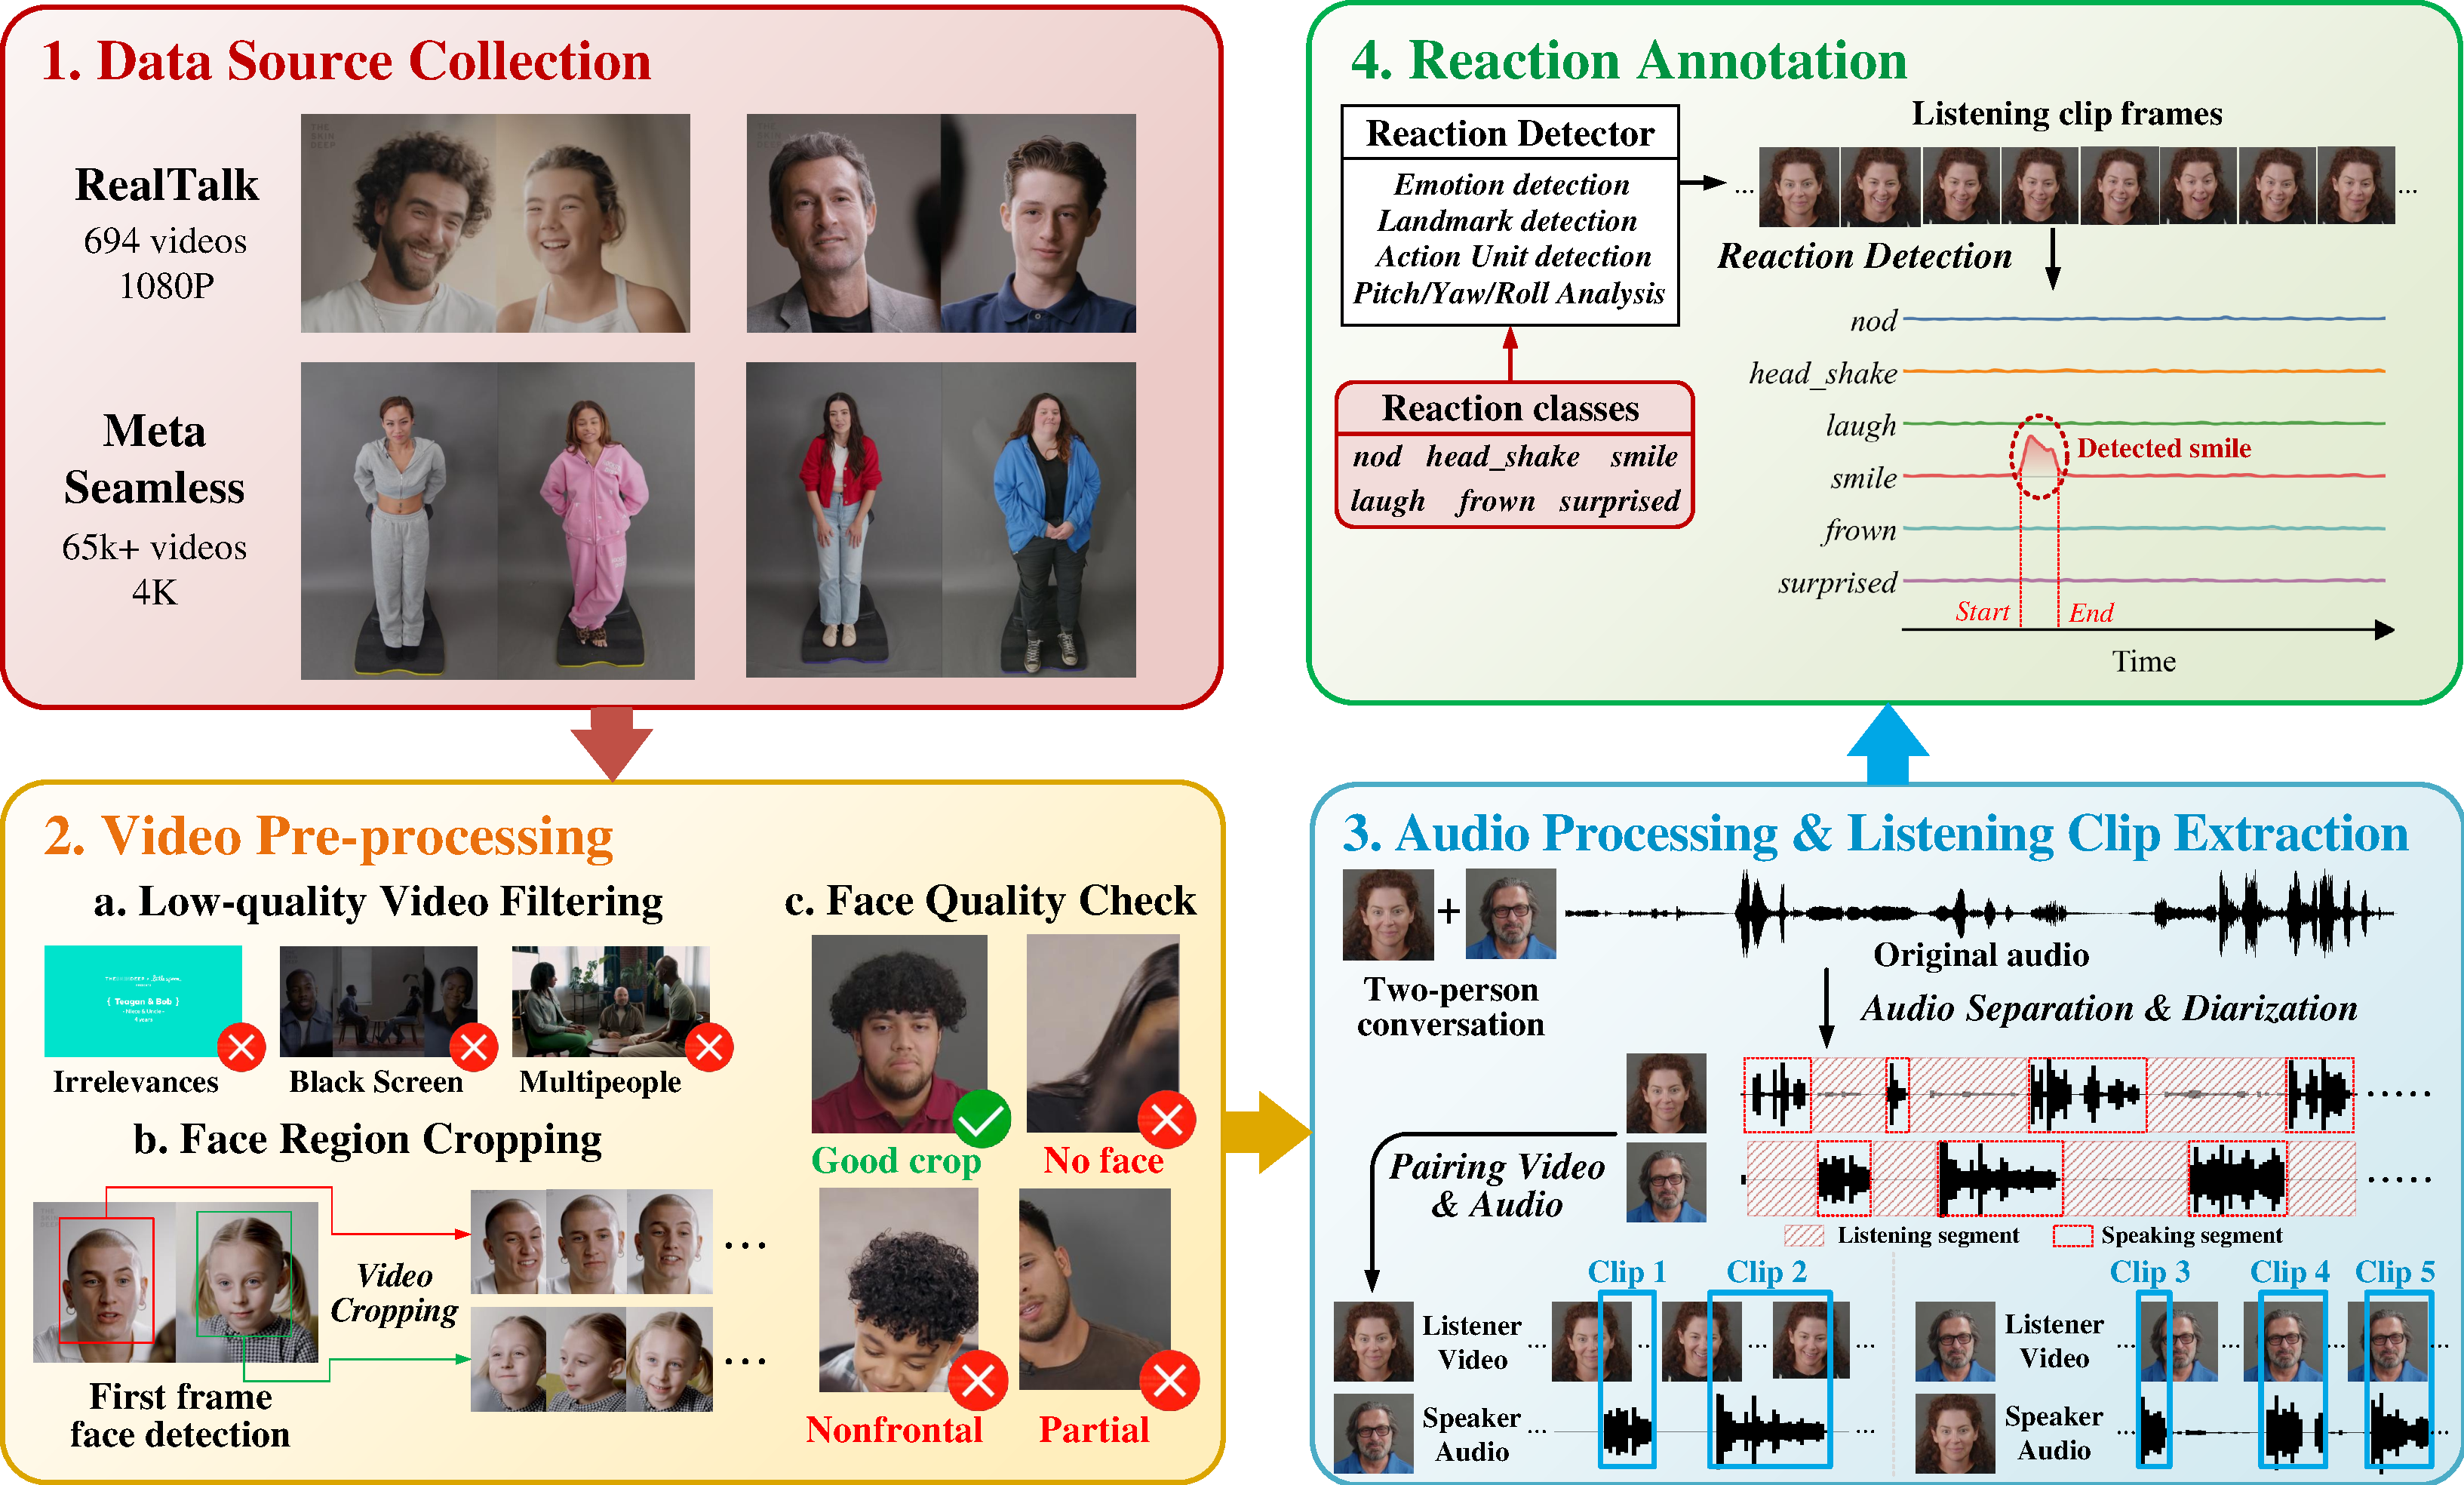
\includegraphics[width=\linewidth,keepaspectratio]{files/curation_pipeline3.pdf}
    \vspace{-1.2em}
    \caption{Overview of our data curation pipeline: \textbf{Step 1}, we leverage conversational data from the RealTalk and Seamless datasets;  \textbf{Step 2}, videos are cropped into facial regions; \textbf{Step 3}, we apply audio separation and diarization to disentangle listening and speaking segments in each conversation with timestamps, and pair speaker audio clips with corresponding listener clips; and \textbf{Step 4}, we define the reaction classes and detect reactions in each paired clip, resulting in multi-class frame-wise reaction annotations.}
    \vspace{-1.2em}
    \label{fig:curation_pipeline}
\end{figure}

Our goal is to construct a listening-head-specific dataset that supports not only audio-driven listener head generation, but also fine-grained modeling and evaluation of listener reactions. To this end, we curate dyadic conversational videos into temporally aligned speaker--listener pairs and further annotate the listener's visible reactions as categorized temporal events. The overall pipeline is shown in Fig. \ref{fig:curation_pipeline}. Starting from RealTalk \cite{geng2023affective} and Seamless Interaction \cite{agrawal2025seamless}, we obtain 107,149 speaker audio/listener-video pairs, corresponding to approximately 147 hours of data.





\subsection{Speaker--Listener Clip Construction}  \label{sec:clip_construction}

As shown in Fig.\ref{fig:curation_pipeline} (2) and (3), we first process the raw dyadic videos to obtain high-quality portrait clips for both conversational participants. Since the original videos may contain scene transitions, black frames, irrelevant content, multiple visible people, severe occlusions, or unstable face crops, visual quality filtering is performed before clip extraction. For retained videos, each participant is cropped into a portrait-centered video and an additional manual face-quality check is conducted to remove clips with missing, partial, or poorly framed faces. This step ensures that the resulting listener videos contain stable facial regions suitable for motion generation and reaction annotation.

We then parse the speaking and listening roles over time. For RealTalk, where the two speakers may be mixed in the original audio, we perform audio separation, denoising, and speaker diarization to estimate participant-level speech activity. For Seamless Interaction, we use the provided high-quality audio streams and diarization results, with timestamp correction when necessary. Based on the resulting speech-activity timelines, each dyadic conversation is decomposed into speaker-dominant intervals. For each interval, we pair the active speaker's audio with the temporally synchronized portrait video of the other participant, who is treated as the listener. This produces paired training examples in the form of speaker audio and listener video, while preserving the conversational timing between the two participants.

Implementation details of speaker-listener clip reconstruction, including filtering criteria, face-crop procedure, diarization correction, and quality-control procedures, are provided in Appendix \ref{app:data_curation}.








\subsection{Reaction Taxonomy and Annotation}  \label{sec:reaction_taxonomy}

A central objective of our dataset is to explicitly capture listener reactions that are semantically meaningful and temporally localized. We focus on six common reaction categories: \textit{nodding}, \textit{head shaking}, \textit{smiling}, \textit{laughing}, \textit{frowning}, and \textit{surprised}, which are visually recognizable and frequently associated with conversational feedback and affective responses \cite{ng2022learning,zhou2022vico,geng2023realtalk}. Compared with micro-behaviors (e.g., eye blinking or gaze shifts), and background motions (e.g., subtle pose adjustments), these reactions have four desirable properties: they convey clear communicative or affective intent, are visually recognizable and are strongly correlated with the conversational context. These properties make them suitable targets for reaction-aware listener generation and reaction-centric evaluation.

As shown in Fig.\ref{fig:curation_pipeline} (4), to annotate listener reactions at scale, we design a visual reaction detector to the cropped listener videos. % with \cite{bulat2017far,goodfellow2013challenges,lugaresi2019mediapipe}. 
For a listener clip with $T$ frames, the detector outputs a dense reaction score vector $\mathbf{r} \in [0,1]^{T \times 6}$, where each channel corresponds to one of the six reaction categories. The detector combines head-motion cues, facial landmark dynamics, facial expression cues, and temporal smoothing to estimate frame-wise reaction confidence. 
% Continuous high-confidence regions are then converted into event-level annotations $\mathcal{A} = \{(y_i, r_i, t_{s,i}, t_{e,i})\}_{i=1}^{N}$, where $N$ is the number of all valid reactions in the clip, $y_i$ denotes the reaction type, $r_i$ is the frame-wise reaction score vector for clip between [$t_{s,i}$, $t_{e,i}$], $t_{s,i}$ and $t_{e,i}$ denote the start and end time of the reaction event. 
Continuous high-confidence regions are then converted into event-level annotations
$A=\{(y_i,r_i,t_{s,i},t_{e,i})\}_{i=1}^{N}$, where $y_i\in\mathcal{Y}$ is the
event type from the six reaction classes, $r_i$ is the frame-wise reaction score
within $[t_{s,i},t_{e,i}]$, and $t_{s,i}$ and $t_{e,i}$ are the start and end
times. Each final event is assigned a single type, and cross-class overlaps are
resolved by keeping the dominant reaction. The resulting annotations therefore provide both sparse temporal boundaries for event-level evaluation and dense frame-wise scores for reaction-aware training supervision.

We further conduct manual verification to remove unreliable detections and improve annotation quality. The final curated dataset contains 64,557 reaction instances in total. The distribution across reaction categories is summarized in Table \ref{tab:reaction_statistics}. \textit{Smiling} and \textit{head shaking} are the most frequent reaction types, while \textit{surprised} reactions occur less often, reflecting their relatively sparse and context-specific nature in natural conversations. The detailed detector design, including class-specific visual cues, smoothing strategies, event merging rules, and thresholds, can be referred to Appendix~\ref{app:reaction_detector}.



\begin{table}[t]
    \centering
    \fontsize{8pt}{7pt}\selectfont
    \setcellgapes{1.5pt}
    \makegapedcells
    \setlength{\tabcolsep}{2pt} 
    \caption{Statistics of the annotated listener reactions in our curated dataset.}
    \label{tab:reaction_statistics}
    \begin{tabular}{c|cccccc|c}
        \Xhline{1.2pt}
        Reaction type & \textit{nodding} & \textit{head shaking} & \textit{smiling} & \textit{laughing} & \textit{frowning} & \textit{surprised} & Total \\
        \hline
        Count & 10,230 & 12,790 & 15,767 & 8,320 & 9,986 & 7,464 & 64,557 \\
        \Xhline{1.2pt}
    \end{tabular}
    \vspace{-1.5em}
\end{table}